\documentclass[a4paper,12pt]{report}
\pdfoutput=1 % if your are submitting a pdflatex (i.e. if you have
             % images in pdf, png or jpg format)
%\directlua{ require("drawboxes")}
\usepackage{float}
\usepackage{jheppub} % for details on the use of the package, please
                     % see the JHEP-author-manual

\usepackage[T1]{fontenc} % if needed
\usepackage{amsfonts}
%%%%%%%%%%%%%%%%%%%%%%%%
%\usepackage[T1]{fontenc}
%\usepackage[utf8]{inputenc}
\usepackage[labelsep=period]{caption} %para que  "Figura" no tenga 2 puntos finales
%\usepackage{caption}
\usepackage{lmodern}
\usepackage[spanish,es-lcroman,es-nosectiondot]{babel} %Para que en vez de Figure use Figura. Las demas opciones sacan 
%los puntos finales de la numeracion en el indice
\usepackage{wrapfig} % para poner imagenes al costado
%\usepackage{amssymb} % para el simbolo de conjunto de numeros
%\usepackage{hyperref}
\usepackage{graphicx}
%\usepackage{enumerate} % para colocar listas
\usepackage{enumitem} % para sacar el espacio en las listas
%\usepackage{makecell} % usado en el prafacio para los nombres a lo ultimo
\usepackage{multicol} % para dos columnas en un parrafo
%\usepackage{tikz} % para las flechas
%\usepackage{adjustbox} %para mover minipage a la derecha
%\usepackage{amsmath} %para usar align
\usepackage{subdepth} % para que los subindices tengan todos la misma posicion
%\usepackage{float} %para las imagenes
%\usepackage[english]{babel}
%\usepackage{caption} % para sacar los dos puntos despues de Figure X
%\usepackage{geometry} % para sacar el espacio de margenes
\usepackage{capt-of} % El entorno \captionsetup del paquete capt-of permite manejar las leyendas de las figuras sin 
%necesidad de utilizar un entorno flotante, garantizando que la figura permanezca dentro del entorno example.
\usepackage{float} % para poner figuras no desfasadas dentro del entorno example
\usepackage{cases} %para enumerar las ecuaciones con llaves

\def\para{\paragraph{}} %para un salto de linea mas grande

%%%%%%%%%%%%%%



\title{\boldmath Notas de física 1}


%% %simple case: 2 authors, same institution
%% \author{A. Uthor}
%% \author{and A. Nother Author}
%% \affiliation{Institution,\\Address, Country}

% more complex case: 4 authors, 3 institutions, 2 footnotes
\author{Claudia Giribet}

% The "\note" macro will give a warning: "Ignoring empty anchor..."
% you can safely ignore it.

\affiliation{Departamento de Física,\\Facultad de Ciencias Exactas y Naturales, \\Universidad de Buenos Aires.}

% e-mail addresses: one for each author, in the same order as the authors
\emailAdd{first@one.univ}





%\abstract{Abstract...}



%\AtBeginShipout {\directlua{drawboxes.visual_debug()}}
\begin{document}
\maketitle
\flushbottom

\chapter{Cinemática}
La cinemática es la rama de la mecánica que estudia los movimientos sin tener en cuenta las causas que los producen. 
Desde su punto de vista es netamente descriptivo.
\para
Comencemos por definir lo que es movimiento. Se dice que un objeto está en movimiento cuando cambia su posición en el 
tiempo. De igual forma, si su posición no cambia con el tiempo, se dice que está en reposo. Vamos a ver que tanto el 
concepto de movimiento como el de reposo son conceptos absolutos. 
\para
Por ejemplo, supongamos que en una estación hay un 
tren esperando a arrancar. Un pasajero se encuentra asomado a la ventanilla, despidiéndose de alguien en el andén. En 
ese momento, el hombre en el andén observa que el pasajero del tren está en reposo (i.e. no se mueve) respecto de él. 
Otro pasajero, que se encuentra sentado junto al primero, también observa que este se encuentra en reposo respecto de 
él. Es decir, la descripción del estado de movimiento del primer pasajero es la misma tanto para el hombre del andén, 
como para el segundo pasajero. Ahora el tren se pone en marcha. El hombre del andén observa que su amigo en el tren se 
aleja de él (i.e. cambia su posición en el tiempo respecto de él); y, por lo tanto, razona que su amigo está en 
movimiento y él está en reposo. Sin embargo, para el segundo pasajero, el estado de movimiento del primer pasajero 
no ha variado y si varia el del hombre del andén. Entonces el hombre en el andén se esta moviendo respecto de ambos 
pasajeros. ¿Quién tiene razón? Tanto el peatón como el segundo pasajero, lo único que ha cambiado es el punto de vista 
del observador. La moraleja es que para referir a un sistema en movimiento hace falta un observador o sistema de 
referencia. El peatón define al anden como su sistema de referencia, el andén está en reposo respecto de él, por lo 
tanto, cualquier objeto que cambie su posición respecto del andén estará en movimiento respecto de este. El segundo 
pasajero define como sus sistema de referencia al tren y, por lo tanto, el peatón esta en movimiento respecto de él. 
Ninguno de los dos sistemas es absoluto, puede decirse que uno está en reposo y el otro en movimiento pero solo hablando 
en forma relativa (i.e. en reposo o en movimiento respecto de él). Aunque pareciera natural elegir el andén como sistema 
en reposo, observen que este se encuentra moviéndose con la Tierra respecto del Sol, que el Sol se encuentra moviéndose 
respecto de las estrellas y así se podría seguir. 

\paragraph*{Consecuencia} Cuando se habla de un sistema en movimiento, siempre hay que 
referirlo a algún sistema de referencia.

\section{Sistema de referencia y sitema de coordenadas}
Vamos a analizar como se especifica la posición de un objeto. Si el objeto es extenso (por ejemplo, el triángulo de la 
Fig. \ref*{fig:1-1}) el observador $O$ puede elegir
\begin{itemize}[noitemsep]
    \item[a)] Un punto del objeto, y ver a que distancia, dirección y sentido se haya respecto de él. Si elige el punto 
    $A$, lo anterior se puede representar con el vector que va desde $O$ hasta $A$. La variación de la posición de A nos 
    va a estar mostrando como se traslada todo el cuerpo pues A se traslada y todo el cuerpo lo acompaña. En este caso, 
    estamos ante un movimiento de traslación.
    \item[b)] Si el objeto esta girando, lo anterior no basta y hay que dar la orientación del objeto, por ejemplo, como 
    varia la posición de $B$ respecto de $A$. En este caso, estamos ante un movimiento de rotación.
\end{itemize}

\begin{wrapfigure}{l}{0pt} 
    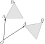
\includegraphics[]{images/f1-1.pdf}
    \caption{}
    \label{fig:1-1}
    \vspace{-20pt}
\end{wrapfigure}

Si el objeto se puede considerar puntual, no tiene sentido hablar de su orientación, o sea no se puede hablar de 
rotación, entonces, el movimiento más general de un objeto puntual es una traslación. Igualmente, si se trata de un 
objeto extenso trasladándose solo basta conocer el movimiento de un punto para conocer el de todos, lo podemos 
considerar puntual. Un ejemplo de esto último es un tren circulando por una vía.

\paragraph{Objeto puntual}
Es aquel cuyas dimensiones son despreciables frente a las distancias típicas del problema. Por 
ejemplo, un avión en vuelo para un observador en tierra.

\para
De acuerdo a (a), la posición se conoce si se conoce el segmento orientado desde el punto de referencia $O$ al punto 
$A$, al cual llamaremos vector posición de $A$. Como el movimiento se realiza en el espacio, conviene plantear un 
sistema de coordenadas para poder describir este vector posición.

\para
Notar que sistema de referencia no es igual a sistema de coordenadas. 

\paragraph{Sistema de referencia}
Sistema al cual se refiere el movimiento.

\paragraph{Sistema de coordenadas}
Se adosa al sistema de referencia para describir el movimiento.

\begin{example}
  Por ejemplo, en la Fig. \ref{fig:1-2} tenemos que $\vec{r}_{\! A}$ da la posición de $A$ desde el sistema de 
  referencia $O$ y $\vec{r}^{\,\prime}_{\!A}$ da la posición de $A$ desde el sistema de referencia $O'$. Entonces 
  estamos cambiando de sistema de referencia.

  \para
  En la Fig. \ref{fig:1-3} tenemos el sistema de referencia $O$ el cual tiene dos sistemas de coordenadas adosados a 
  él, $(x,y,z)$ y $(x',y',z')$. El vector $\vec{r}_{\! A}$ es el mismo pero cambia su descripción. Para el primer 
  sistema de coordenadas tenemos que  
  \begin{equation*}
    \vec{r}_{A}(t) = (x_{A}(t),y_{A}(t),z_{A}(t)) 
  \end{equation*}
  mientras que para el segundo sistema de coordenadas es 
  \begin{align*}
    \vec{r}_{A}(t) = (x^{\prime}_{A}(t),y^{\prime}_{A}(t),z^{\prime}_{A}(t))
  \end{align*}
    \begin{figure}[htbp]
      \centering
      \begin{minipage}[b]{0.4\textwidth}
        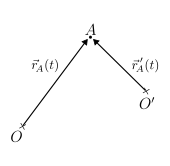
\includegraphics[]{images/f1-2.pdf}
        \caption{}
        \label{fig:1-2}
      \end{minipage}
      \hspace{-0.02\textwidth}
      \begin{minipage}[b]{0.4\textwidth}
        \hspace{15pt}
        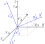
\includegraphics[]{images/f1-3.pdf}
        \caption{}
        \label{fig:1-3}
      \end{minipage}
    \end{figure}
\end{example}

Supongamos un sistema $A$ (Fig.\ref{fig:1-4}) en movimiento respecto del observador $O$. El vector posición sigue a 
$A$ en su movimiento. Su extremo describe la curva que $A$ describe en el espacio. Esa curva se denomina 
\textit{trayectoria} y caracteriza al movimiento.

\begin{figure}[H]
  \centering
  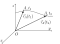
\includegraphics[]{images/f1-4.pdf}
  \caption{}
  \label{fig:1-4}
\end{figure}

%\begin{wrapfigure}{l}{0pt}
%  \includegraphics[]{images/f1-4-bis.pdf}
%  \caption{}
%  \label{fig:1-4}
%  \vspace{-74pt}
%\end{wrapfigure}

Para estudiar el movimiento de traslación nos interesa conocer
\begin{itemize}[noitemsep]
  \item[•] La trayectoria (curva que describe en el espacio).
  \item[•] Magnitudes físicas que lo describen.
  \item[•] Relaciones entre las magnitudes.
\end{itemize}

\section{Grados de libertad y vínculos}
La trayectoria siempre es una curva en el espacio, sin embargo, se observa que no es exactamente lo mismo describir el 
movimiento de:
\begin{itemize}[noitemsep]
 \item[1.] Una mosca moviéndose libremente en la habitación.
 \item[2.] Una mosca moviéndose sobre una mesa.
 \item[3.] Una mosca moviéndose sobre un hilo tenso.
\end{itemize}

En (1) se necesitan tres ejes coordenados para describir el movimiento, mientras que en (2) bastan solo dos y en (3) 
solo uno.

\para
Se dice que un sistema tiene \textit{n grados de libertad} si se requieren n parámetros independientes para fijar su 
posición. Cada grado de libertad corresponde a una posibilidad de movimiento. En el caso de la traslación el movimiento 
puede tener hasta 3 grados de libertad.
¿Cuando se tienen menos? Cuando hay condiciones materiales que limitan el movimiento (vínculos). Ejemplo: una hormiga 
se mueve sobre la superficie de una piedra. Esa superficie esta caracterizada por $z=f(x,y)$. Entonces tengo 2 
parámetros independientes ($x$ e $y$), o sea, 2 grados de libertad.

\section{Movimiento unidimensional rectilíneo}
En el espacio, basta con trabajar con un eje cartesiano. Si la trayectoria es una recta (Fig. \ref{fig:1-5}), 
entonces hacemos coincidir el eje de coordenadas con la trayectoria. Con este sistema de coordenadas nuestro vector 
posición es $\vec{r}(t) = x(t)\hat{x}$.
\begin{figure}[htbp]
  \centering
  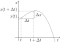
\includegraphics[]{images/f1-6.pdf}
  \caption{}
  \label{fig:1-5}
\end{figure}

\para
Podemos representar (Fig. \ref{fig:1-6}) cómo varía $x(t)$. Esta va a ser nuestra curva paramétrica u horaria de la 
trayectoria.
\begin{figure}[htbp]
  \centering
  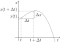
\includegraphics[]{images/f1-6.pdf}
  \caption{}
  \label{fig:1-6}
\end{figure}

Supongamos que se quiere conocer la rapidez con que cambia la posición con $t$.
Al tiempo $t$, el móvil se encuentra en $x(t)$. Un $\Delta t$ después, al tiempo $t+\Delta t$, se encuentra en 
$x(t+\Delta t)$. Defino que, en ese $\Delta t$, la \textit{rapidez media} fue
\begin{align*}
  \langle \vec{v}_x\rangle =\frac{\Delta x}{\Delta t}\hat{x}=\frac{x(t+\Delta t)- x(t)}{\Delta t} \hat{x}
\end{align*}
A esa \textit{rapidez media} se la llama \textit{velocidad media}.

\para
Si queremos saber la rapidez con que cambia instante a instante, afinamos la medición tomando un $\Delta t$ cada vez más 
chico.
\begin{align*}
  \lim\limits_{\Delta t \rightarrow 0}\displaystyle\frac{x(t+\Delta t)- x(t)}{\Delta t} \hat{x}\equiv 
  \frac{dx(t)}{dt}\hat{x}\equiv\dot{x}(t)\hat{x}=v_{x}(t)\hat{x}
\end{align*}
$v_{x}(t)$ se llama la \textit{velocidad instantánea} (o velocidad a secas) en la dirección $x$. Observemos que su valor 
es igual a la pendiente de la recta tangente a la curva horaria en cada punto. 

\para
Veamos sus características: 
\begin{itemize}[noitemsep]
  \item [•]La velocidad es un vector. En general vamos a ver que
  \begin{equation*}
    \vec{v}(t)=\frac{d\vec{r}(t)}{dt}
  \end{equation*}
  En nuestro caso (movimiento unidimensional)
  \begin{align*}
    \vec{v}(t)=\frac{dx(t)}{dt}\hat{x} 
  \end{align*}
  donde $\hat{x}$ marca la dirección del movimiento, $dt$ es la rapidez con que cambia la coordenada y $dx$ es el 
  sentido del movimiento.
  \item [•] La velocidad es tangente a la trayectoria punto a punto. Queda claro que es tangente a la curva horaria.
  Tambien podemos ver que es tangente a la trayectoria (ver Fig. \ref{fig:1-7}).
  \begin{align*}
    \vec{v}(t)&=\lim\limits_{\Delta t\rightarrow 0}\frac{\vec{r}(t+\Delta t)-\vec{r}(t)}{\Delta t} \\
    \vec{v}(t)&=\lim\limits_{\Delta t\rightarrow 0}\frac{\Delta\vec{r}}{\Delta t}
  \end{align*}

  Entonces $\vec{v}$ es paralelo a $\Delta \vec{r}$ y $\Delta\vec{r}$ es tangente a la 
  curva cuando $\Delta t\rightarrow 0$.
  \begin{figure}[htbp]
    \centering
    \includegraphics[]{images/f1-7.pdf}
    \caption{}
    \label{fig:1-7}
  \end{figure}
\end{itemize}

\begin{example}
  Supongamos que $x(t)$ varia segun la Fig. \ref{fig:1-8}

  \begin{figure}[H]
    \centering
    \includegraphics[]{images/f1-8.pdf}
    \caption{}
    \label{fig:1-8}
  \end{figure}
  
  Del gráfico anterior vemos que (por el valor de la pendiente en cada punto)
  \begin{align*}
    &v_{A},v_{B}>0, \ \ v_{A}>v_{B}\\
    &v_{C}=0 \\
    &v_{D},v_{E}<0, \ \ \left|v_{E}\right|>\left|v_{D}\right|    
  \end{align*}
\end{example}

De la misma manera podemos definir la rapidez media e instantánea con que cambia la velocidad. Esa rapidez se 
denomina \textit{aceleración}. Siguiendo el mismo proceso que antes resulta que
\begin{align*}
  \vec{a}(t)&=\frac{d\vec{v}(t)}{dt}=\frac{d^{2}\vec{r}(t)}{dt^{2}}\\
  \vec{a}(t)&=\dot{\vec{v}}(t)=\ddot{\vec{r}}(t)
\end{align*}

En nuestro caso (movimiento unidimensional)
\begin{align*}
  \vec{a}_{x}(t)=\dot{v_{x}}\hat{x}=\ddot{x}\hat{x}
\end{align*}
Por analogía con lo anterior, vemos que la aceleración es tangente a la curva $v(t)$ en cada punto.

\begin{example}
  Supongamos que $v(t)$ varía como se muestra en la Fig. \ref{fig:1-9}.
  \begin{figure}[H]
    \centering
    \includegraphics[]{images/f1-9.pdf}
    \caption{}
    \label{fig:1-9}
  \end{figure}

  Del gráfico anterior vemos que (por el valor de la pendiente en cada punto)
  \begin{align*}
    &a_{A},a_{B}>0, \ \ a_{A}> a_{B}\\
    &a_{C}=0 \\
    &a_{D},a_{E}<0, \ \ \left|a_{E}\right|>\left|a_{D}\right|    
  \end{align*}

  Tenemos que para todo tiempo $t$, la velocidad $v$ es mayor o igual a 
  cero. Esto implica que el móvil avanza hacia los $x$ positivos para todo $t$. Sin embargo
  \begin{align*}
    &t_{A}<t<t_{C}: a>0 \Longrightarrow v \text{ aumenta}\\
    &t_{C}<t<t_{E}: a<0 \Longrightarrow v \text{ disminuye}
  \end{align*}
  
  Representando la trayectoria
  \begin{figure}[H]
    \centering
    \includegraphics[]{images/f1-10.pdf}
    \caption{\textquestiondown Qué pasa en $E$? En $E$ se detiene.}
    \label{fig:1-10}
  \end{figure}
  
  La aceleración con igual sentido que la velocidad aumenta ésta, mientras que una aceleración contraria a la velocidad 
  disminuye su módulo. Es un error decir que una aceleración negativa disminuye la velocidad; que la velocidad aumente 
  o disminuya depende del sentido relativo de la aceleración.
  
  \begin{multicols}{2}
    \hspace{10pt}
    $\left.\begin{array}{rcl}
    \vec{a} \longrightarrow\\ 
    \vec{v} \longrightarrow 
    \end{array}\right\}$ $\vec{v}$ aumenta
    
    \noindent
    $\left.\begin{array}{rcl}
    \vec{a} \longrightarrow\\ 
    \vec{v} \longleftarrow 
    \end{array}\right\}$ $\vec{v}$ disminuye
  \end{multicols}
  
  \begin{multicols}{2}
    \hspace{10pt}
    $\left.\begin{array}{rcl}
    \vec{a} \longleftarrow\\ 
    \vec{v} \longrightarrow 
    \end{array}\right\}$ $\vec{v}$ disminuye
    
    \noindent
    $\left.\begin{array}{rcl}\vec{a} \longleftarrow\\ 
    \vec{v} \longleftarrow \end{array}\right\}$ $\vec{v}$ aumenta
  \end{multicols}
\end{example}

En general, si conocemos $\vec{v}(t)= v(t)\hat{x}$, podemos llegar a conocer $x(t)$
\begin{align*}
  \vec{v}(t) &= v(t)\hat{x} = \frac{dx(t)}{dt}\hat{x} \Longrightarrow v(t) = \frac{dx(t)}{dt} \Longrightarrow
  v(t) dt = dx(t)
\end{align*}

Integramos esta última igualdad
\begin{align*}
  \int\limits_{x(t_0)}^{x(t)}dx(t) &= \int\limits_{t_0}^{t}v(t)dt \\
  x(t) &= x(t_0) + \int\limits_{t_0}^{t}v(t)dt
\end{align*}

Notemos que
\begin{itemize}[noitemsep]
  \item [•] $t_0$ es el instante en que comienza el movimiento, o bien en que comienza la observación del movimiento.
  \item [•] $x(t_0)$ es la posición del móvil al instante $t_0$.
  \item [•] El origen del tiempo puede elegirse de acuerdo a cada problema en particular. Por ejemplo, $t_0 = 0$.
\end{itemize}

\para
Si conocemos $\vec{a}(t) = a(t)\hat{x}$
\begin{align*}
  a(t) = \frac{dv(t)}{dt} \Longrightarrow dv(t) = a(t)dt
\end{align*}
Integramos
\begin{align*}
  \int\limits_{v(t_0)}^{v(t)}dv(t) &= \int\limits_{t_0}^{t}a(t)dt \\
  v(t) &= v(t_0) + \int\limits_{t_0}^{t}a(t)dt
\end{align*}

\subsection{Movimiento rectilíneo uniforme (MRU)}
Está caracterizado por
\begin{align*}
  \begin{cases}
    \vec{v}(t) = \vec{cte} \\
    \vec{a}(t) = \vec{0}
  \end{cases}
\end{align*}

Hacemos coincidir al eje $x$ con la dirección del movimiento. Entonces
\begin{align*}
  \vec{v}(t) = v_0 \hat{x} \Longrightarrow \frac{dx}{dt} = v_0 \Longrightarrow dx = v_0 dt
\end{align*}

Integramos
\begin{align*}
  \int\limits_{x(t_0)}^{x(t)} dx = \int\limits_{t_0}^{t}v_0 dt \\
  x(t) = x(t_0) + v_0(t-t_0)
\end{align*}

si $x(t_0) = x_0$, llegamos a
\begin{align*}
  x(t) = x_0 + v_0(t-t_0)
\end{align*}

Representemos $x(t)$, $v(t)$ y $a(t)$ para el caso particular donde $x_0 > 0$ y $v_0 > 0$
\begin{figure}[H]
  \centering
  \includegraphics[]{images/f1-11.pdf}
  \caption{}
\end{figure}

\subsection{Movimiento rectilíneo uniformemente variado (MRUV)}
Caracterizado por $\vec{a}(t) = \vec{cte}$ (en módulo, dirección y sentido). Nuevamente hacemos coincidir al eje $x$ con
 la dirección de movimiento
\begin{align*}
  \vec{a}(t) &= \frac{d\vec{v}}{dt} \Longrightarrow a_0 \hat{x} = \frac{dv}{dt} \hat{x} \Longrightarrow 
  a_0 = \frac{dv}{dt} \Longrightarrow dv = a_0 dt
\end{align*}

Integramos para obtener $v(t)$
\begin{align*}
  \int\limits_{v(t_0)}^{v(t)} dv &= \int\limits_{t_0}^{t}a_0 dt \\
  v(t) &= v_0 + a_0(t-t_0)
\end{align*}
donde $v_0 = v(t_0)$. Integramos $v(t)$ para obtener $x(t)$
\begin{align*}
  \frac{dx}{dt} &= v(t) \Longrightarrow dx = v(t)dt \\
  \int\limits_{x(t_0)}^{x(t)}dx &= \int\limits_{t_0}^{t}v(t)dt = \int\limits_{t_0}^{t}[v_0 + a_0(t-t_0)]dt \\
  x(t) &= x_0 + v_0(t-t_0) + \frac{1}{2}a_0(t-t_0)^2
\end{align*}
donde $t_0$ es el instante en que comienza el movimiento o éste comienza a observarse, $x_0$ es es la posición del móvil
 a $t=t_0$ y $v_0$ es la velocidad del móvil a $t=t_0$.

\para
Representemos $x(t)$, $v(t)$ y $a(t)$ para el caso particular donde $x_0,v_0,a_0 > 0$

\begin{figure}[htbp]
  \centering
  \includegraphics[]{images/f1-12.pdf}
  \caption{}
\end{figure}

\subsection{Caída libre}
Un caso muy imporante del \textit{MRUV} lo constituye la caída de los cuerpos bajo la acción de la atracción 
gravitatoria. Se debe a Galileo el descubrimiento que todos los cuerpos que están cerca de la superficie de la Tierra 
caen hacia ella con una aceleración constante, dirigida hacia el centro de la Tierra, independiente de la forma, tamaño 
y material que los compone. Esta acelaración se denomina \textit{aceleración de la gravedad} y la denotamos con 
$\vec{g}$. El valor de $\vec{g}$ depende del lugar de la Tierra y la altura sobre el nivel del mar. A nivel del mar 
$\left|\vec{g}\right| = 9.8 \ m/s^2$.

\para
Supongamos un cuerpo que a $t=0$ se lo deja caer desde una altura $h$ con una velocidad inicial 
$\vec{v}_0 = -v_0\hat{z}$. De acuerdo a lo que vimos
\begin{align*}
  z(t) &= z(t=0) + v_z(t=0)t + \frac{1}{2}a_z t^2 \\
  v_z(t) &= v_z(t=0) + a_zt
\end{align*}

Según los datos del problema
\begin{align*}
  z(t=0) &= h, \ v_z (t=0) = -v_0, \ a_z = -g
\end{align*}
Entonces
\begin{align*}
  z(t) &= h -v_0t-\frac{1}{2}g t^2 \\
  v_z(t) &= -v_0-g t
\end{align*}
En particular, si se lo lanza sin una velocidad inicial ($v_0=0$)
\begin{align*}
  z(t) &= h -\frac{1}{2}g t^2 \\
  v_z(t) &= -g t
\end{align*}

Si queremos saber el tiempo que tarda en caer desde $h$ hasta el suelo, podemos
plantear $z(t=t_c) =0$, donde $t_c$ es el tiempo de caída.
\begin{align*}
  z(t_c) = 0 = h -\frac{1}{2}g t^2_c \\
  t_c = \sqrt{\frac{2h}{g}}
\end{align*}

La velocidad con que llega al suelo es
\begin{align*}
  v(t_c) &= -gt_c = -\sqrt{2hg}
\end{align*}

\begin{figure}[H]
  \centering
  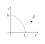
\includegraphics[]{images/f1-13.pdf}
  \caption{}
\end{figure}

\section{Movimiento en 3 dimensiones}
El móvil describe una trayectoria general en el espacio (Fig. \ref{fig:1-14}). El vector posición sigue a $P$ en su 
movimiento; su extremo describe la curva que $P$ describe en el espacio (trayectoria), la cual caracteriza al 
movimiento.

\begin{figure}[htbp]
  \centering
  \includegraphics[]{images/f1-14.pdf}
  \caption{}
  \label{fig:1-14}
\end{figure} 
\para
Si se elige una terna de ejes coordenados $(x,y,z)$, la posición del objeto se puede descomponer como una suma de 3 
vectores (ver Fig.(\ref{fig:1-15})). Las proyecciones de $\skew{-2.0}\vec{r}_P(t)$ en el sistema de ejes es
\begin{align}
  \vec{r}_P(t) &= \vec{x}_P(t) + \vec{y}_P(t) + \vec{z}_P(t) \nonumber \\ 
  \vec{r}_P(t) &=  x_P(t) \hat{x} + y_P(t) \hat{y} + z_P(t) \hat{z}
  \label{eq:1-2}
\end{align}
Por lo tanto, la posición del objeto queda determinada en cada instante dando 3 datos.

\begin{figure}[htbp]
  \centering
  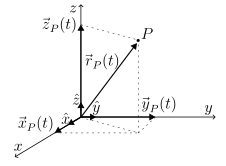
\includegraphics[]{images/f1-15.pdf}
  \caption{}
  \label{fig:1-15}
\end{figure}

Esto permite descomponer el movimiento en 3 \textit{movimientos unidimensionales independientes} (en realidad, solo 
ligados a través de $t$). Entonces la Ec.(\ref{eq:1-2}) se descompone en 3 ecuaciones escalares, llamadas ecuaciones 
paramétricas de la trayectoria o curvas horarias.

\begin{example}
Supongamos un móvil moviendóse (Fig. \ref{fig:1-16}) de tal manera que sus curvas horarias son 
\begin{align}
  \begin{cases}
    x(t) = v t  \\ 
    y(t) = k t^2
  \end{cases}
  \label{eq:1-3}
\end{align}
donde $v$ y $k$ son constantes.

\begin{figure}[htbp]
  \centering
  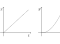
\includegraphics[]{images/f1-16.pdf}
  \caption{}
  \label{fig:1-16}
\end{figure}

Queremos encontrar la trayectoria $y(x)$. \textquestiondown Qué nos dice la Ec.(\ref{eq:1-3})? Nos dice que para cada 
instante $t$ (el mismo instante), el móvil se encuentra en un punto del plano de coordenadas $(x,y) = (vt,kt^2)$.

\para
El móvil alcanza el valor $x$ en $t=x/v$. En ese momento, su posición en $y$ será
\begin{align*}
y\left(t=\frac{x}{v}\right) &= k\left(\frac{x}{v}\right)^2 \\
y(x) &= \frac{k}{v^2}x^2
\end{align*}
la cuál es una trayectoria parabólica (ver Fig.(\ref{fig:1-17})). Observemos que $y$ varía cuadraticamente, mientras que 
$x$ varía linealmente.
\begin{figure}[htbp]
  \centering
  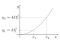
\includegraphics[]{images/f1-17.pdf}
  \caption{$x_1 = vt_1$ y $x_2 = 2vt_1$}
  \label{fig:1-17}
\end{figure}

\end{example}

Lo mismo se puede hacer con la velocidad y la aceleración. Habiamos visto que
\begin{align*}
  \vec{v}(t) &= \frac{d\skew{-1}\vec{r}(t)}{dt} = \dot{\skew{-1}\vec{r}}(t) \\
  \vec{v}(t) &= \dot{x}\hat{x} + \dot{y}\hat{y} + \dot{z}\hat{z}
\end{align*}
Entonces las ecuaciones paramétricas (o curvas horarias) de la velocidad son

\begin{align*}
  \begin{cases}
    v_x(t) = \dot{x}(t)  \\ 
    v_y(t) = \dot{y}(t) \\
    v_z(t) = \dot{z}(t)
  \end{cases}
\end{align*}

Para el caso de la aceleración
\begin{align*}
\vec{a}(t) &= \dot{\skew{-1}\vec{v}}(t) = \ddot{\skew{-1}\vec{r}}(t) \\
\vec{a}(t) &= \dot{v}_x\hat{x} + \dot{v}_y\hat{y} + \dot{v}_z\hat{z} \\
\vec{a}(t) &= \ddot{x}\hat{x} + \ddot{y}\hat{y} + \ddot{z}\hat{z}
\end{align*}
Entonces las ecuaciones paramétricas (o curvas horarias) de la aceleración son
\begin{align*}
\begin{cases}
a_x(t) = \ddot{x}(t) \\ 
a_y(t) = \ddot{y}(t)\\
a_z(t) = \ddot{z}(t)
\end{cases}
\end{align*}

Notar que cada coordenada (cada movimiento unidireccional) varía con su propia velocidad y aceleración.

\section{Tiro oblicuo en el vacío}
Supongamos que se arroja un objeto con una cierta velocidad inicial $\skew{-1}\vec{v}_0$, desde el suelo. La aceleración
 presente es la de la gravedad, $\vec{g}$. La velocidad $\skew{-1}\vec{v}_0$ y $\vec{g}$ están contenidas en un mismo 
plano, entonces todo el movimiento se desarrollará en ese plano. Caracterizamos al plano con 2 ejes cartesianos 
$x$ e $y$, y vamos a descomponer el movimiento según esos ejes.
\begin{figure}[H]
  \centering
  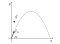
\includegraphics[]{images/f1-18.pdf}
  \caption{}
\end{figure}

Según nuestro sistema de ejes
\begin{align*}
  \begin{cases}
    a_x =0 \\
    a_y = -g
  \end{cases}
\end{align*}
y nuestro vector aceleración es
\begin{align*}
  \vec{a} = -g \hat{y}
\end{align*}

Entonces en la dirección $x$ tendremos un MRU pues la acelaración en esa dirección es cero, y en la dirección de $y$ 
tendremos un MRUV pues la aceleración en esa dirección es constante.

\para
Escribamos el vector posición
\begin{align*}
  \skew{-1}\vec{r}(t) = x(t)\hat{x}+ y(t)\hat{y}
\end{align*}
donde
\begin{align*}
  x(t) &= x_0 + v_{0x}(t-t_0)\\
  y(t) &= y_0 + v_{0y}(t-t_0) + \frac{1}{2}a_y (t-t_0)^2
\end{align*}
Eligiendo $t_0 = 0$, $x_0 = y_0 = 0$ y reemplazando el valor de la aceleración en $y$
\begin{align*}
  x(t) &= v_{0x}t\\
  y(t) &= v_{0y}t - \frac{1}{2}g t^2
\end{align*}

¿Cuánto vale la velocidad inicial?
Si $|\vec{v}_0| = v_0$, tenemos que
\begin{align*}
  \vec{v}_0 &= v_{0x}\hat{x} + v_{0y} \hat{y} \\
  \vec{v}_0 &= v_0 \cos(\alpha)\hat{x} + v_0 \sen({\alpha})\hat{y}
\end{align*}

\begin{figure}[htbp]
  \centering
  \includegraphics[]{images/f1-19-bis.pdf}
  \caption{}
\end{figure}

Entonces
\begin{numcases}{}
  x(t) = v_0 \cos(\alpha)t \label{eq:1-4} \\
  y(t) = v_0 \sen(\alpha)t -\frac{1}{2}g t^2 \label{eq:1-5}
\end{numcases}

\begin{numcases}{\hspace{-13pt}}
  v_y(t) = v_0 \sen(\alpha) - gt \label{eq:1-6} \\
  v_x(t) = v_0 \cos(\alpha) \nonumber
\end{numcases}

\begin{numcases}{\hspace{-68pt}}
  a_x(t) = 0 \nonumber \\
  a_y(t) = -g \nonumber
\end{numcases}

\vspace{12pt}
¿Qué tipo de trayectoria describe? Despejamos $t$ de la Ec.(\ref{eq:1-4})
\begin{equation*}
  x = v_0 \cos(\alpha)t \Longrightarrow t = \frac{x}{v_0 \cos(\alpha)}
\end{equation*} 
Reemplazamos $t$ en la Ec.(\ref{eq:1-5}) y obtenemos una parábola
\begin{equation*}
  y(x) = x \tg(\alpha)-\frac{1}{2} \frac{g}{v_0^2\cos^2(\alpha)}x^2
\end{equation*}

\para
Vamos a encontrar algunas características de la trayectoria:
\begin{enumerate}
  \item Altura máxima $H$ que alcanza el móvil. Está caracterizada porque corresponde a tener $v_y = 0$.
  Sea $t_H$ el instante tal que $v_y(t_H) = 0$. Evaluamos la Ec.(\ref{eq:1-6}) en $t_H$
  \begin{align*}
    v_y(t_H) = v_0 \sen(\alpha) - gt_H &= 0 \Longrightarrow t_H = \frac{v_0 \sen(\alpha)}{g}
  \end{align*}
  Por lo tanto
  \begin{align*}
    y(t_H) = H &= v_0\sen(\alpha)t_H -\frac{1}{2}g t_H^2 \\
    H &= v_0\sen(\alpha)\frac{v_0 \sen(\alpha)}{g} -\frac{1}{2}g \left(\frac{v_0 \sen(\alpha)}{g}\right)^2 \\
    H &= \frac{1}{2}\frac{v_0^2\sen(\alpha)^2}{g}
  \end{align*}
  \item Alcance máximo $L$ que alcanza el móvil. Está caracterizado porque corresponde a tener $y = 0$. Sea $t_L$ el 
  instante tal que $y(t_L) = 0$. Evaluamos la Ec.(\ref{eq:1-5}) en $t_L$
  \begin{align*}
    y(t_L) = v_0\sen(\alpha)t_L -\frac{1}{2}g t_L^2 = 0 
    \Longrightarrow &t_L \left(v_0\sen(\alpha) -\frac{1}{2}g t_L \right) = 0 \\ 
    \Longrightarrow &t_L = 0 \lor t_L = \frac{2v_0 \sen(\alpha)}{g}
  \end{align*}
  Por lo tanto
  \begin{align*}
    x(t_L) = L &= \frac{2 v_0 \cos(\alpha) \sen(\alpha)}{g} \\
    L &= \frac{v_0^2}{g}\sen(2\alpha)         
  \end{align*}

  \begin{figure}[htbp]
    \centering
    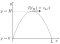
\includegraphics[]{images/f1-20.pdf}
    \caption{}
    \label{fig:1-20}
  \end{figure}
\end{enumerate}

\paragraph{Observación}






% The bibliography will probably be heavily edited during typesetting.
% We'll parse it and, using the arxiv number or the journal data, will
% query inspire, trying to verify the data (this will probalby spot
% eventual typos) and retrive the document DOI and eventual errata.
% We however suggest to always provide author, title and journal data:
% in short all the informations that clearly identify a document.

\begin{thebibliography}{99}

\bibitem{a}
Author, \emph{Title}, \emph{J. Abbrev.} {\bf vol} (year) pg.

\bibitem{b}
Author, \emph{Title},
arxiv:1234.5678.

\bibitem{c}
Author, \emph{Title},
Publisher (year).


% Please avoid comments such as "For a review'', "For some examples",
% "and references therein" or move them in the text. In general,
% please leave only references in the bibliography and move all
% accessory text in footnotes.

% Also, please have only one work for each \bibitem.
\end{thebibliography}
\end{document}

